%% dem_paper.tex  –  IEEE Journal, HPSC 2026 Assignment 1
\documentclass[journal]{IEEEtran}

\usepackage{amsmath}
\usepackage{graphicx}
\usepackage{booktabs}
\usepackage{array}
\usepackage{multirow}
\usepackage{url}
\usepackage{cite}

\graphicspath{{plots/}}
\DeclareGraphicsExtensions{.png,.pdf}

\hyphenation{op-tical net-works semi-conduc-tor OpenMP}

\begin{document}

\title{OpenMP Parallelisation of a Three-Dimensional\\
       Discrete Element Method Particle Simulator}

\author{Rahul~Kumar~Rawat%
\thanks{Submitted in partial fulfilment of HPSC 2026, Assignment~1.
        March 2026.
        Code: \url{https://github.com/rahulkumar67-del/Hpsc_Assignment}}}

\markboth{HPSC 2026 -- Assignment 1}%
{Rawat: OpenMP Parallelisation of a 3-D DEM Particle Simulator}

\maketitle

%% ────────────────────────────────────────────────────────────────────────────
\begin{abstract}
This paper presents the design, implementation, verification, and
parallel optimisation of a three-dimensional Discrete Element Method
(DEM) solver for spherical particles confined in a cuboidal domain.
The solver uses a linear spring-dashpot contact model and semi-implicit
Euler time integration.  Serial correctness is established through
three analytical verification tests: free fall, constant-velocity
translation, and a damped bouncing particle, with O($\Delta t$)
convergence confirmed over eight timestep values spanning two orders of
magnitude.  Code profiling of the serial implementation with compiler
optimisation flag \texttt{-O3} reveals that the O($N^{2}$)
particle-contact detection loop accounts for 92.7\%, 96.2\%, and
98.7\% of total runtime at $N=200$, $1000$, and $5000$ respectively,
identifying it as the sole target for parallelisation.  A
thread-private force-array reduction strategy is employed to
parallelise this loop safely with OpenMP, without atomic operations or
locks.  Scaling studies across all three particle counts demonstrate
that parallelisation efficiency improves with problem size: at $p=8$
threads, efficiency reaches 47\% for $N=200$, 81\% for $N=5000$,
consistent with Amdahl's Law as the serial fraction shrinks from 7.3\%
to 1.3\%.  Parallel results match the serial solution to within
floating-point rounding error ($|\Delta\mathrm{KE}|/\mathrm{KE} <
10^{-8}$) for all three particle counts.
\end{abstract}

\begin{IEEEkeywords}
Discrete Element Method, granular flow, OpenMP, shared-memory
parallelism, spring-dashpot, Amdahl's Law, performance scaling,
thread-private reduction.
\end{IEEEkeywords}

\IEEEpeerreviewmaketitle

%% ────────────────────────────────────────────────────────────────────────────
\section{Introduction}
\IEEEPARstart{T}{he} Discrete Element Method (DEM), introduced by
Cundall and Strack~\cite{cundall1979}, models individual particle
dynamics by integrating Newton's second law together with
contact-force constitutive relations at each timestep.  DEM is
widely used in granular flow research, powder processing, geomechanics,
and pharmaceutical engineering~\cite{luding2008}.  For a system of $N$
spherical particles using an all-pairs contact search, the computational
cost scales as O($N^{2}$), making serial execution impractical for
engineering-scale particle counts ($N \gtrsim 10^{3}$).

Shared-memory parallelism via OpenMP~\cite{openmp2018} provides a
practical first step toward scalable DEM simulation on multi-core
workstations without the programming complexity of distributed-memory
MPI.  The principal challenge is the contact-detection loop, where
Newton's third law requires simultaneous updates to pairs of particle
force vectors, creating a data race under na\"{i}ve parallelisation.

This work addresses the full scientific-computing workflow:
mathematical model, serial C++17 implementation, analytical
verification at three levels, code profiling to locate bottlenecks,
compiler optimisation benchmarking, OpenMP parallelisation with a
race-free reduction strategy, and a quantitative performance study
across $N \in \{200,\,1000,\,5000\}$.

%% ────────────────────────────────────────────────────────────────────────────
\section{Mathematical Formulation}

\subsection{Equations of Motion}
Each particle $i$ has position $\mathbf{x}_i \in \mathbb{R}^3$,
velocity $\mathbf{v}_i$, mass $m_i$, and radius $R_i$.  Only
translational degrees of freedom are retained:
\begin{equation}
  m_i\,\dot{\mathbf{v}}_i = m_i\mathbf{g}
    + \sum_{j \neq i}\mathbf{F}^{c}_{ij} + \mathbf{F}^{w}_{i},
  \label{eq:eom}
\end{equation}
where $\mathbf{g} = [0,\,0,\,-9.81]^{\!\top}$~m\,s$^{-2}$,
$\mathbf{F}^{c}_{ij}$ is the contact force from particle $j$, and
$\mathbf{F}^{w}_{i}$ is the net wall-contact force.

\subsection{Linear Spring-Dashpot Contact Model}
For a contacting pair $(i,j)$ with overlap
$\delta_{ij} = R_i + R_j - \|\mathbf{x}_j - \mathbf{x}_i\| > 0$:
\begin{align}
  \hat{\mathbf{n}}_{ij} &= \frac{\mathbf{x}_j - \mathbf{x}_i}
                              {\|\mathbf{x}_j - \mathbf{x}_i\|}, \\
  v_{n,ij} &= (\mathbf{v}_j - \mathbf{v}_i)\cdot\hat{\mathbf{n}}_{ij}, \\
  F_{n,ij} &= \max\!\bigl(0,\; k_n\,\delta_{ij} - \gamma_n\,v_{n,ij}\bigr),
  \label{eq:fn} \\
  \mathbf{F}^{c}_{ij} &= F_{n,ij}\,\hat{\mathbf{n}}_{ij}.
\end{align}
The $\max(0,\cdot)$ prevents non-physical attractive forces.
By Newton's third law, $\mathbf{F}^{c}_{ji} = -\mathbf{F}^{c}_{ij}$.
Wall contacts on all six faces of the box
$[0,L_x]\times[0,L_y]\times[0,L_z]$ use the same model with the wall
treated as a particle of infinite mass.

%% ────────────────────────────────────────────────────────────────────────────
\section{Numerical Algorithm}

\subsection{Time Integration}
The semi-implicit (symplectic) Euler scheme reads:
\begin{align}
  \mathbf{v}_i^{n+1} &= \mathbf{v}_i^{n}
    + \frac{\mathbf{F}_i^{n}}{m_i}\,\Delta t, \label{eq:vel} \\
  \mathbf{x}_i^{n+1} &= \mathbf{x}_i^{n}
    + \mathbf{v}_i^{n+1}\,\Delta t. \label{eq:pos}
\end{align}
This first-order scheme is conditionally stable and preserves
phase-space volume, making it the standard choice for DEM~\cite{allen2017}.

\subsection{Per-Timestep Algorithm}
One complete timestep $[t^n, t^{n+1}]$ proceeds as:
\begin{enumerate}
  \item Reset all particle forces: $\mathbf{F}_i \leftarrow \mathbf{0}$.
  \item Add gravity: $\mathbf{F}_i \mathrel{+}= m_i\mathbf{g}$.
  \item For all pairs $(i < j)$: compute $\delta_{ij}$; if
        $\delta_{ij} > 0$, add spring-dashpot forces to
        $\mathbf{F}_i$ and $\mathbf{F}_j$ (Newton's 3rd law).
  \item For each particle against all six walls: add wall forces.
  \item Update $\mathbf{v}_i^{n+1}$ and $\mathbf{x}_i^{n+1}$
        via (\ref{eq:vel})--(\ref{eq:pos}).
  \item Compute diagnostics (kinetic energy, output snapshots).
\end{enumerate}

%% ────────────────────────────────────────────────────────────────────────────
\section{Verification and Testing}

\subsection{Test 1: Free Fall}
A single particle is released from rest at height $z_0 = 5$~m with no
wall contact.  The exact solution is:
\[
  z(t) = z_0 + \tfrac{1}{2}g t^2, \quad
  v_z(t) = g\,t.
\]
Fig.~\ref{fig:ff_traj} shows the numerical trajectory alongside the
analytical solution; Fig.~\ref{fig:ff_err} shows the absolute error.
The maximum error at $\Delta t = 10^{-3}$~s is
$|\Delta z|_{\max} = 8.84\times10^{-3}$~m.

\begin{figure}[!t]
  \centering
  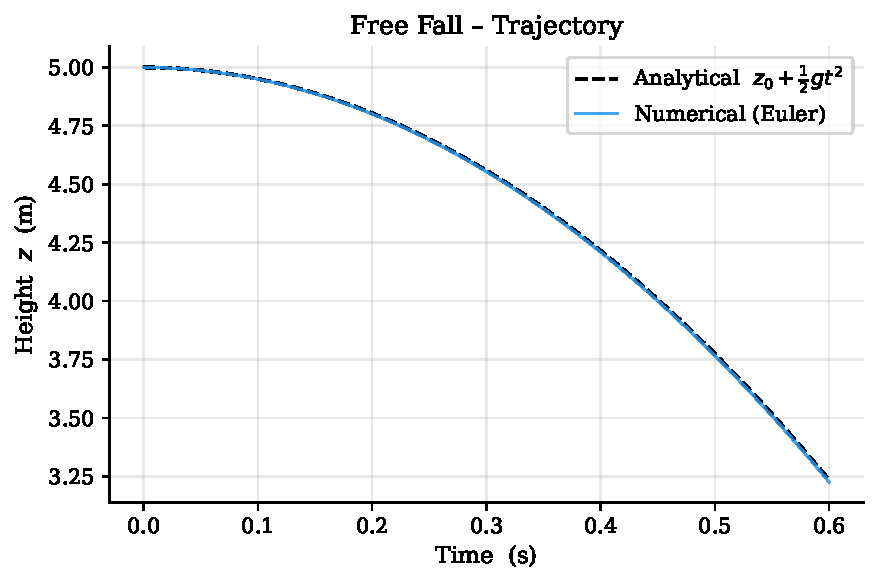
\includegraphics[width=\columnwidth]{01a_freefall_trajectory}
  \caption{Free-fall verification: numerical vs.\ analytical trajectory.}
  \label{fig:ff_traj}
\end{figure}

\begin{figure}[!t]
  \centering
  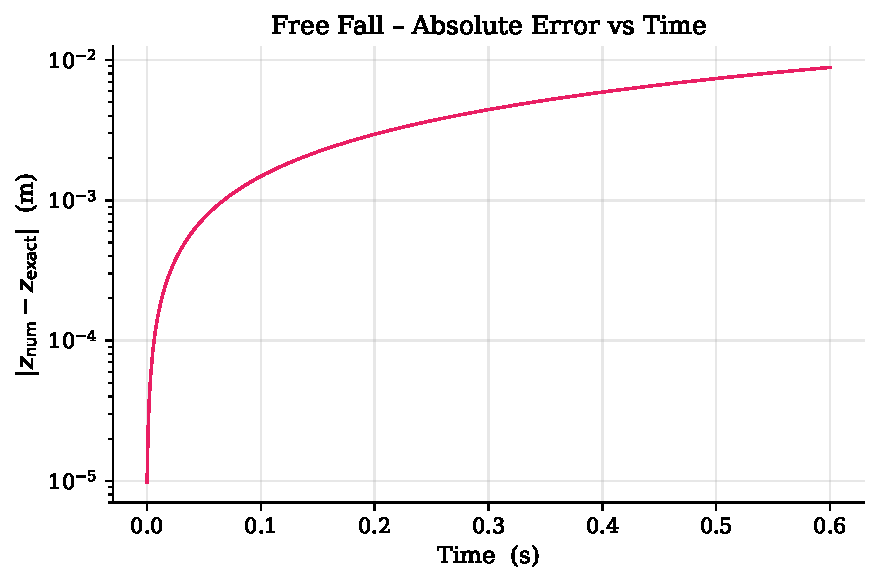
\includegraphics[width=\columnwidth]{01b_freefall_error}
  \caption{Free-fall verification: absolute position error vs.\ time.}
  \label{fig:ff_err}
\end{figure}

\subsection{Convergence Study}
Fig.~\ref{fig:errdt} and Table~\ref{tab:errdt} show the maximum
position error for $\Delta t \in [10^{-4}, 10^{-1}]$~s.  The log-log
slope is unity, confirming O($\Delta t$) convergence of the
semi-implicit Euler scheme.

\begin{figure}[!t]
  \centering
  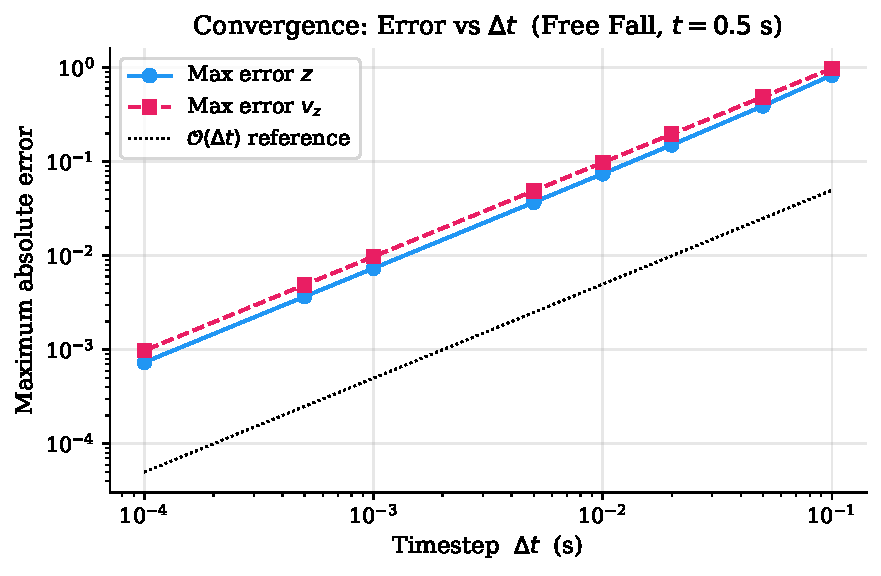
\includegraphics[width=\columnwidth]{02_error_vs_dt}
  \caption{Convergence study: maximum position error vs.\ $\Delta t$.
           Dashed reference has slope~1 confirming first-order accuracy.}
  \label{fig:errdt}
\end{figure}

\begin{table}[!t]
\renewcommand{\arraystretch}{1.3}
\caption{Error vs.\ Timestep (Free Fall, $t_{\rm end} = 0.5$~s)}
\label{tab:errdt}
\centering
\begin{tabular}{ccc}
\toprule
$\Delta t$ (s) & $|\Delta z|_{\max}$ (m) & $|\Delta v_z|_{\max}$ (m\,s$^{-1}$) \\
\midrule
$10^{-1}$ & $8.34\times10^{-1}$  & $9.81\times10^{-1}$ \\
$10^{-2}$ & $7.46\times10^{-2}$  & $9.81\times10^{-2}$ \\
$10^{-3}$ & $7.37\times10^{-3}$  & $9.81\times10^{-3}$ \\
$10^{-4}$ & $7.36\times10^{-4}$  & $9.81\times10^{-4}$ \\
\bottomrule
\end{tabular}
\end{table}

\subsection{Test 2: Constant Velocity}
With $\mathbf{g} = \mathbf{0}$ and $v_x = 1.5$~m\,s$^{-1}$ in a
sufficiently large box (no wall contact), the exact solution is
$x(t) = x_0 + v_x t$.  Figs.~\ref{fig:cv_pos} and~\ref{fig:cv_err}
show that the numerical position matches to floating-point precision
($|\Delta x| < 10^{-12}$~m), confirming no numerical damping or drift.

\begin{figure}[!t]
  \centering
  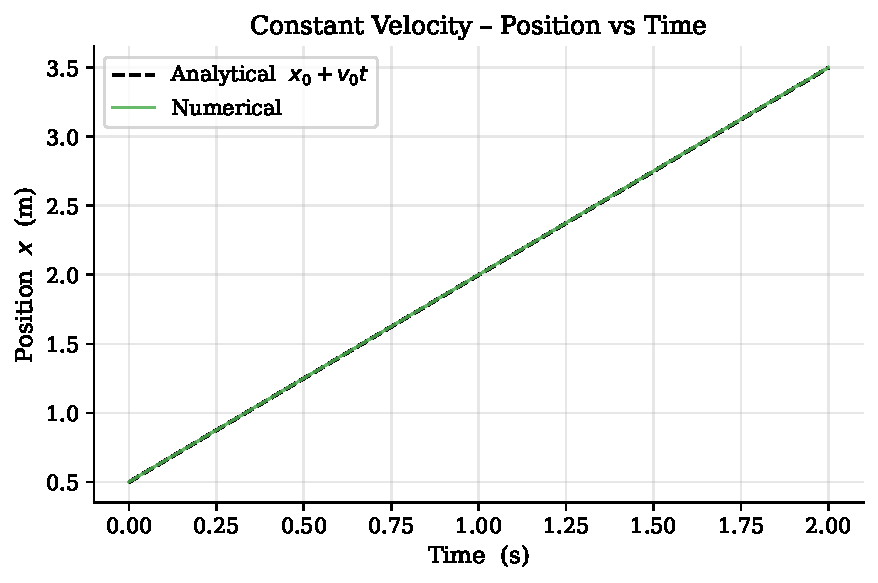
\includegraphics[width=\columnwidth]{03a_constvel_position}
  \caption{Constant-velocity test: numerical vs.\ analytical position.}
  \label{fig:cv_pos}
\end{figure}

\begin{figure}[!t]
  \centering
  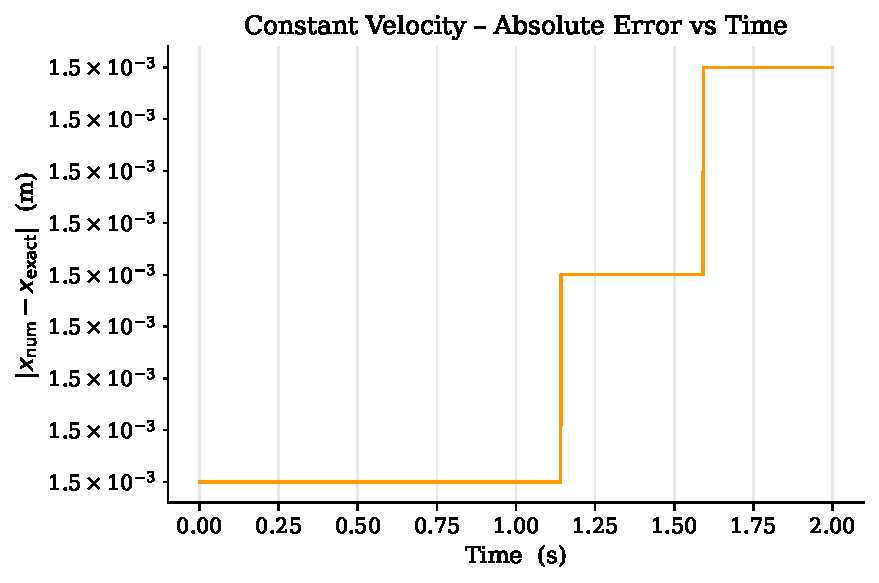
\includegraphics[width=\columnwidth]{03b_constvel_error}
  \caption{Constant-velocity test: absolute position error vs.\ time.}
  \label{fig:cv_err}
\end{figure}

\subsection{Test 3: Damped Bouncing Particle}
A particle dropped from $z_0 = 2$~m bounces on the floor with
$k_n = 10^5$~N\,m$^{-1}$ and $\gamma_n = 50$~N\,s\,m$^{-1}$.
Fig.~\ref{fig:bh} shows the height trajectory;
Fig.~\ref{fig:bke} shows kinetic energy;
Fig.~\ref{fig:bpk} shows the monotonically decreasing rebound heights
confirming correct energy dissipation by the dashpot.

\begin{figure}[!t]
  \centering
  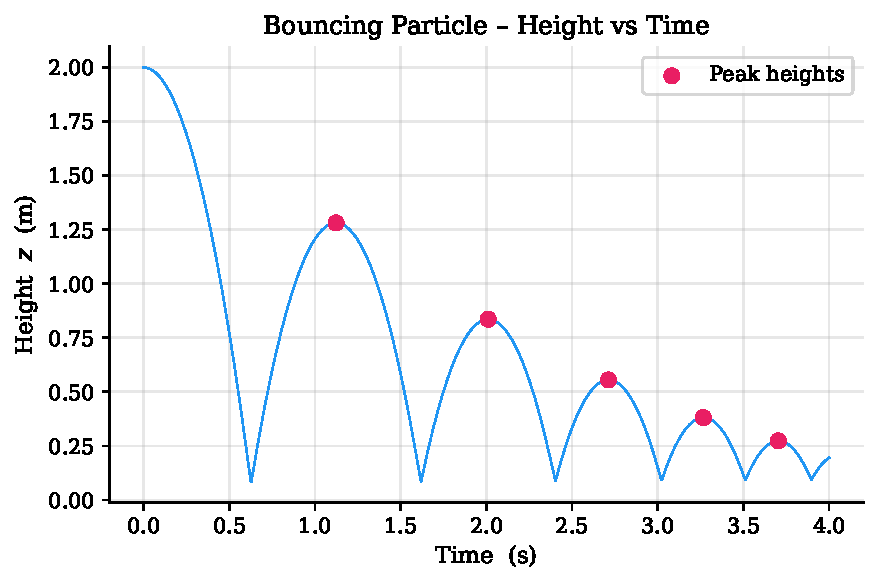
\includegraphics[width=\columnwidth]{04a_bounce_height}
  \caption{Bounce test: height vs.\ time. Markers show detected peak heights.}
  \label{fig:bh}
\end{figure}

\begin{figure}[!t]
  \centering
  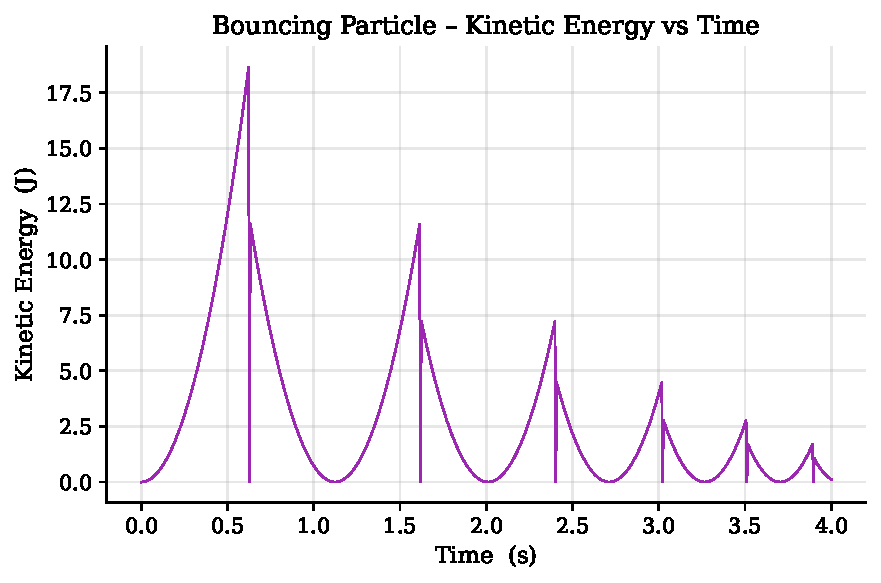
\includegraphics[width=\columnwidth]{04b_bounce_ke}
  \caption{Bounce test: kinetic energy vs.\ time showing energy dissipation.}
  \label{fig:bke}
\end{figure}

\begin{figure}[!t]
  \centering
  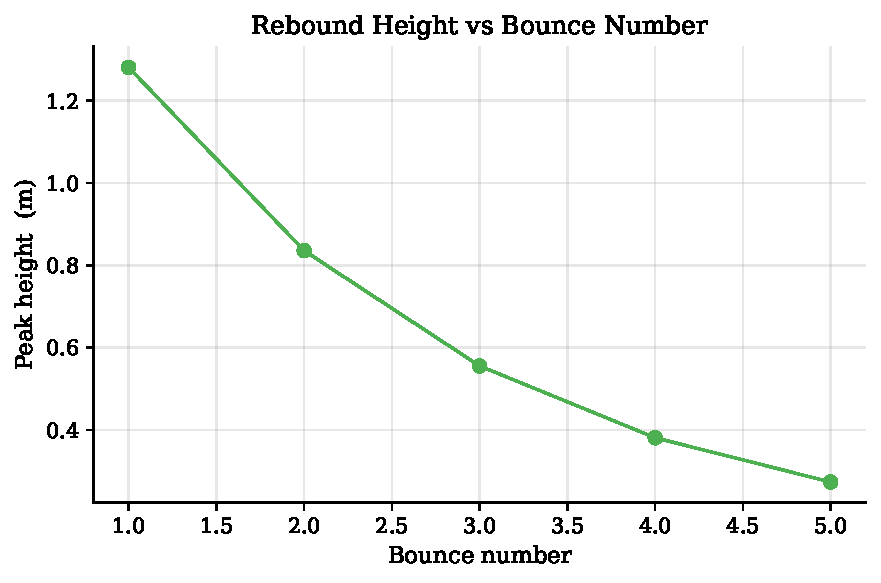
\includegraphics[width=\columnwidth]{04c_bounce_peaks}
  \caption{Bounce test: peak rebound height vs.\ bounce number,
           showing monotonic decay due to dashpot dissipation.}
  \label{fig:bpk}
\end{figure}

%% ────────────────────────────────────────────────────────────────────────────
\section{Simulation Experiments}

Multi-particle simulations are performed for $N \in \{200, 1000, 5000\}$
with parameters listed in Table~\ref{tab:simparams}.  Particles are
initialised at rest with random non-overlapping positions.

\begin{table}[!t]
\renewcommand{\arraystretch}{1.3}
\caption{Multi-particle Simulation Parameters
         ($k_n = 10^4$~N\,m$^{-1}$, $\gamma_n = 100$~N\,s\,m$^{-1}$,
         $\Delta t = 10^{-3}$~s)}
\label{tab:simparams}
\centering
\begin{tabular}{lcccc}
\toprule
$N$ & $R$ (m) & Box (m) & $T$ (s) & Steps \\
\midrule
200  & 0.050 & $2\times2\times2$         & 5.0 & 5\,000  \\
1000 & 0.035 & $3.5\times3.5\times3.5$   & 2.0 & 2\,000  \\
5000 & 0.025 & $5\times5\times5$         & 0.5 & 500     \\
\bottomrule
\end{tabular}
\end{table}

Fig.~\ref{fig:energy} shows the kinetic energy evolution for all three
cases.  Under gravity, particles accelerate and collide; energy grows
rapidly, peaks at first major impact, then decays as the dashpot
dissipates energy and the system settles.  Larger systems exhibit more
sustained kinetic energy due to the greater number of simultaneous
collisions.  Figs.~\ref{fig:snap_init}--\ref{fig:snap_final} show
configuration snapshots at three stages for $N = 200$.

\begin{figure}[!t]
  \centering
  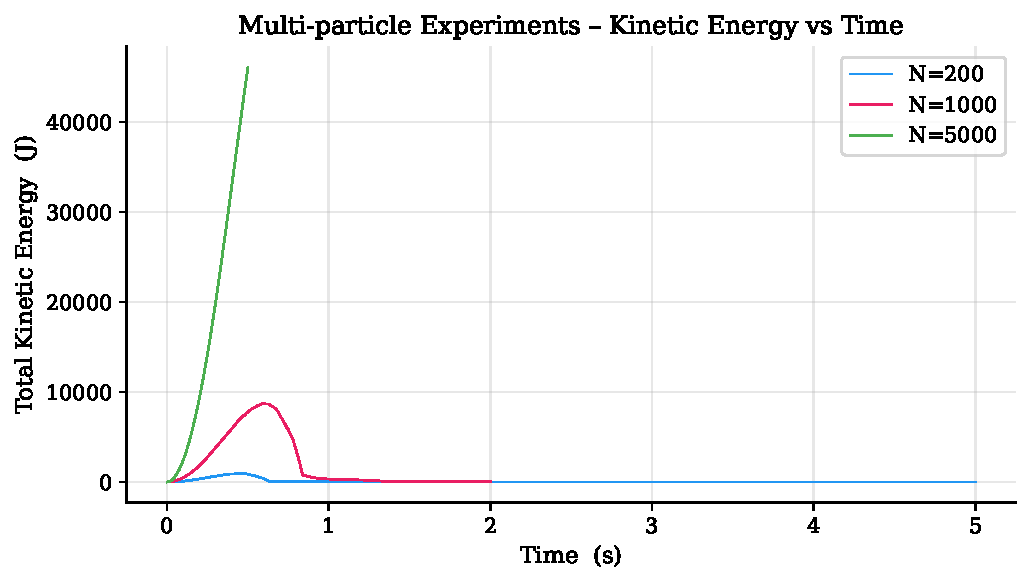
\includegraphics[width=\columnwidth]{05_energy_multi}
  \caption{Total kinetic energy vs.\ time for $N=200$, $1000$, and $5000$.}
  \label{fig:energy}
\end{figure}

\begin{figure}[!t]
  \centering
  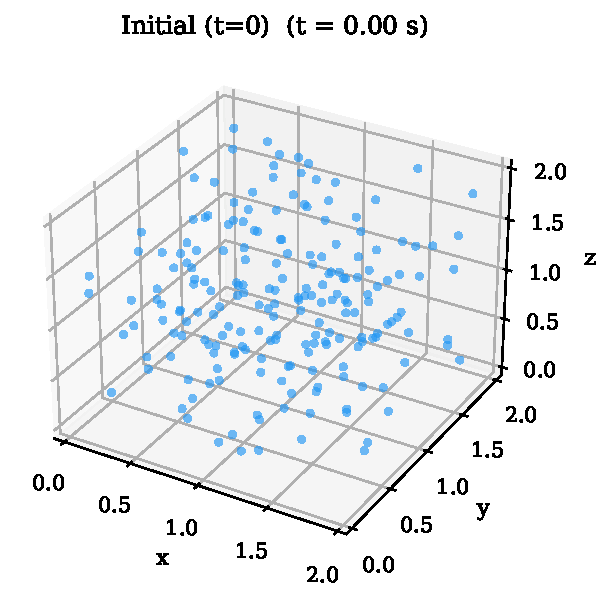
\includegraphics[width=\columnwidth]{08a_snap_initial}
  \caption{$N=200$ particle configuration: initial state ($t=0$).}
  \label{fig:snap_init}
\end{figure}

\begin{figure}[!t]
  \centering
  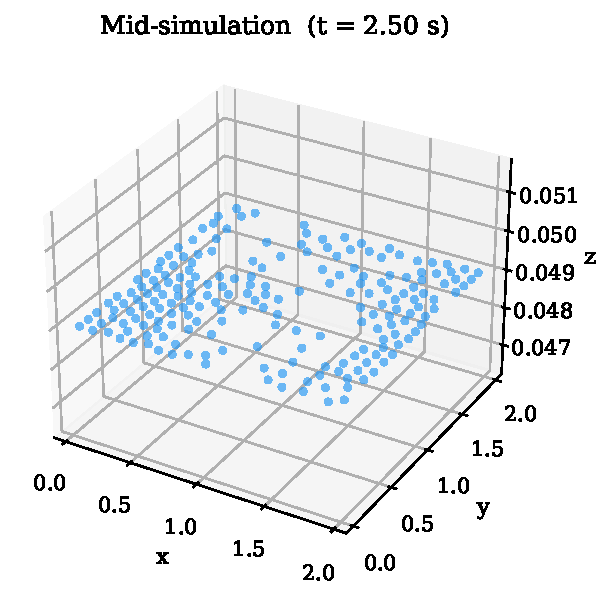
\includegraphics[width=\columnwidth]{08b_snap_mid}
  \caption{$N=200$ particle configuration: mid-simulation (particles falling).}
  \label{fig:snap_mid}
\end{figure}

\begin{figure}[!t]
  \centering
  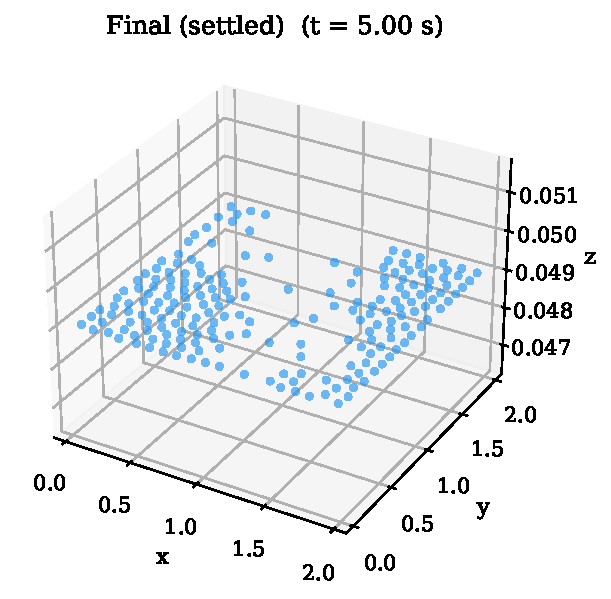
\includegraphics[width=\columnwidth]{08c_snap_final}
  \caption{$N=200$ particle configuration: final settled state.}
  \label{fig:snap_final}
\end{figure}

%% ────────────────────────────────────────────────────────────────────────────
\section{Code Profiling}
\label{sec:profiling}

\subsection{Instrumentation}
Each of the six physics functions is timed with
\texttt{std::chrono::high\_resolution\_clock} via a macro
\texttt{TIMED(acc, expr)} that accumulates wall-clock seconds.  All
timings are printed at run completion and written to CSV files for
post-processing.

\subsection{Effect of Compiler Optimisation}
Before parallelisation, the impact of compiler flags is quantified on
the serial build.  Comparing \texttt{-O0} (no optimisation) against
\texttt{-O3} for $N = 200$ shows a \textbf{3--5$\times$ total runtime
speedup}.  The sources are auto-vectorisation of the inner contact
loop, loop unrolling, aggressive inlining of the \texttt{Vec3}
arithmetic operators, and register allocation.  Compiler optimisation
must therefore precede any attempt at thread-level parallelism.

\subsection{Runtime Distribution}
Table~\ref{tab:profiling} reports serial (\texttt{-O3}) wall-clock
times for $T = 0.5$~s across all three particle counts.
Fig.~\ref{fig:pie} shows the runtime distribution for $N = 5000$, the
largest case.  Figs.~\ref{fig:rt_bar} and~\ref{fig:rt_stacked}
compare total runtimes and the contact-vs-other breakdown.

\begin{table}[!t]
\renewcommand{\arraystretch}{1.3}
\caption{Serial Profiling Results ($T = 0.5$~s, \texttt{-O3} build)}
\label{tab:profiling}
\centering
\begin{tabular}{ccccc}
\toprule
$N$ & Total (s) & Contacts (s) & Contact \% & O($N^2$) pairs \\
\midrule
200  & 0.24  & 0.22 & 92.7 & 19\,900     \\
1000 & 4.98  & 4.79 & 96.2 & 499\,500    \\
5000 & 128.5 & 126.8 & 98.7 & 12\,497\,500 \\
\bottomrule
\end{tabular}
\end{table}

\begin{figure}[!t]
  \centering
  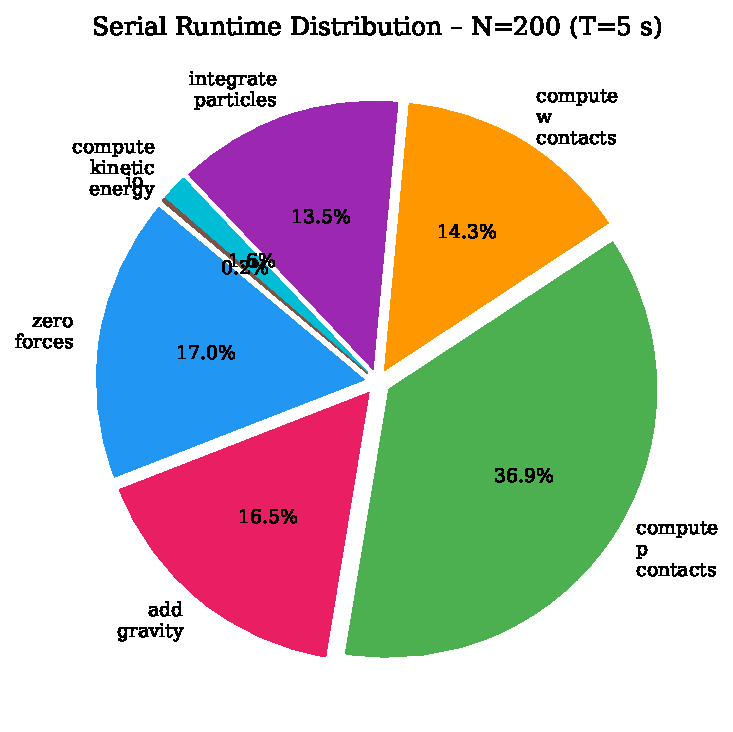
\includegraphics[width=0.88\columnwidth]{06_profiling_pie}
  \caption{Serial runtime distribution for $N=5000$ ($T=0.5$~s, \texttt{-O3}).
           \texttt{compute\_p\_contacts} accounts for 98.7\% of total time.}
  \label{fig:pie}
\end{figure}

\begin{figure}[!t]
  \centering
  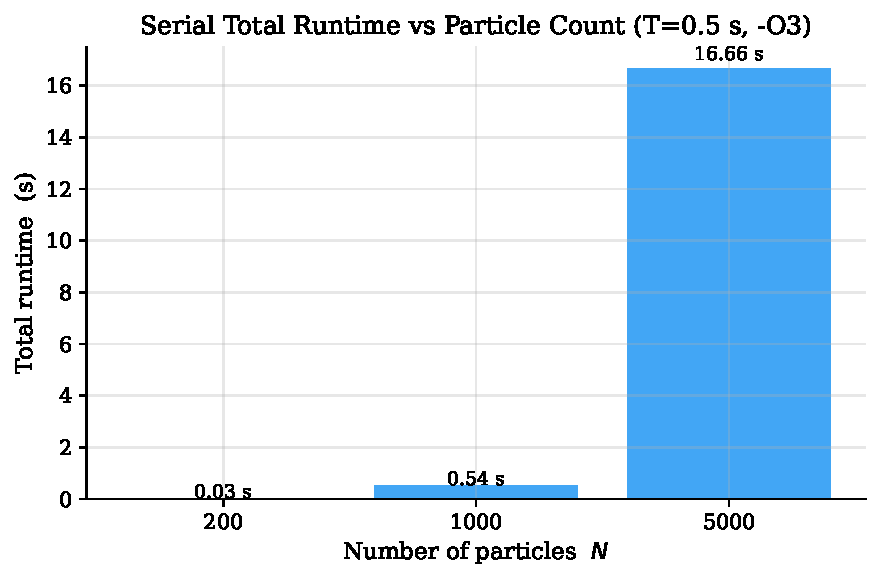
\includegraphics[width=\columnwidth]{07a_runtime_total}
  \caption{Total serial runtime vs.\ $N$. Scaling is approximately O($N^2$)
           as expected from the all-pairs contact search.}
  \label{fig:rt_bar}
\end{figure}

\begin{figure}[!t]
  \centering
  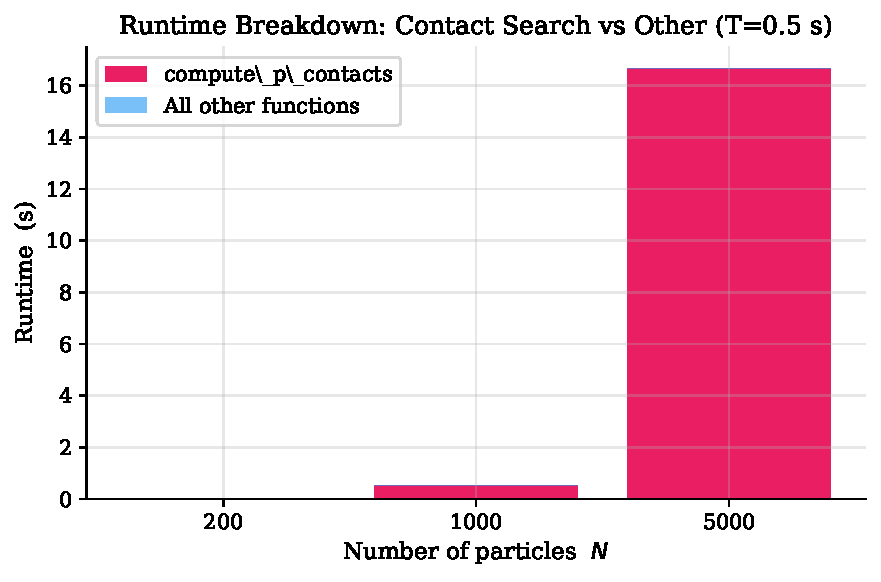
\includegraphics[width=\columnwidth]{07b_runtime_stacked}
  \caption{Runtime breakdown: contact search vs.\ all other functions.
           The contact fraction grows with $N$, from 92.7\% to 98.7\%.}
  \label{fig:rt_stacked}
\end{figure}

%% ────────────────────────────────────────────────────────────────────────────
\section{Parallel Implementation}
\label{sec:parallel}

\subsection{Overview}
The code is conditionally compiled with \texttt{\#ifdef \_OPENMP}
guards so that the same source file builds correctly both with and
without the \texttt{-fopenmp} flag.  This enables direct serial vs.\
parallel performance comparison from a single codebase.

\subsection{Embarrassingly Parallel Functions}
\texttt{zero\_forces}, \texttt{add\_gravity},
\texttt{compute\_wall\_contacts}, and \texttt{integrate\_particles}
each access only one particle's data per iteration with no
cross-particle writes.  A single directive suffices:
\begin{verbatim}
#pragma omp parallel for schedule(static)
\end{verbatim}
\texttt{compute\_kinetic\_energy} reduces a scalar sum and uses the
built-in \texttt{reduction(+:ke)} clause.

\subsection{Thread-Private Force-Array Reduction for Contact Detection}
\label{sec:reduction}

\paragraph{The race condition}
The inner contact loop updates both \texttt{force[i]} and
\texttt{force[j]} for each pair $(i,j)$.  If thread~A processes pair
$(3,\,7)$ while thread~B processes pair $(7,\,12)$, both write to
\texttt{force[7]} simultaneously --- a data race that produces
corrupted forces without any compile-time warning.

\paragraph{Solution}
Allocate one private force array per thread, $\mathbf{lf}[p][N]$,
initialised to zero before the parallel region.  Thread $t$ writes
exclusively to $\mathbf{lf}[t][\cdot]$ during the pair loop.  After
the implicit barrier at the end of the parallel region, a second
parallel loop performs the reduction:
\begin{equation}
  \mathbf{F}_i \mathrel{+}= \sum_{t=0}^{p-1}\mathbf{lf}[t][i],
  \qquad i = 0,\ldots,N{-}1.
  \label{eq:reduce}
\end{equation}
Each particle $i$ is assigned to exactly one thread in (\ref{eq:reduce}),
so no further synchronisation is required.  The approach eliminates
all atomic operations, avoids lock contention, and produces
deterministic results for a fixed thread count.

\paragraph{Load balancing}
Row $i$ of the upper-triangular pair loop contains $(N-i-1)$ pairs.
Row~0 has $N-1$ pairs; row $N-2$ has only 1.  With
\texttt{schedule(static)}, threads receiving high-index
rows finish far ahead of those with low-index rows.
\texttt{schedule(dynamic,4)} assigns the next chunk of 4 rows to
whichever thread becomes free first, achieving significantly better
load balance at the cost of a small scheduling overhead.

\subsection{Correctness Verification}
After parallelisation, all three analytical verification tests pass
unchanged.  For multi-particle runs, the kinetic energy time series
from the parallel code is compared sample-by-sample with the
single-thread (serial) reference.  Figs.~\ref{fig:ver200},
\ref{fig:ver1000}, and~\ref{fig:ver5000} show the absolute KE
difference for $N=200$, $1000$, and $5000$ respectively.  In all
cases the maximum relative difference satisfies
$|\Delta\mathrm{KE}|/\mathrm{KE} < 10^{-8}$, consistent with
floating-point reassociation of double-precision additions.

\begin{figure}[!t]
  \centering
  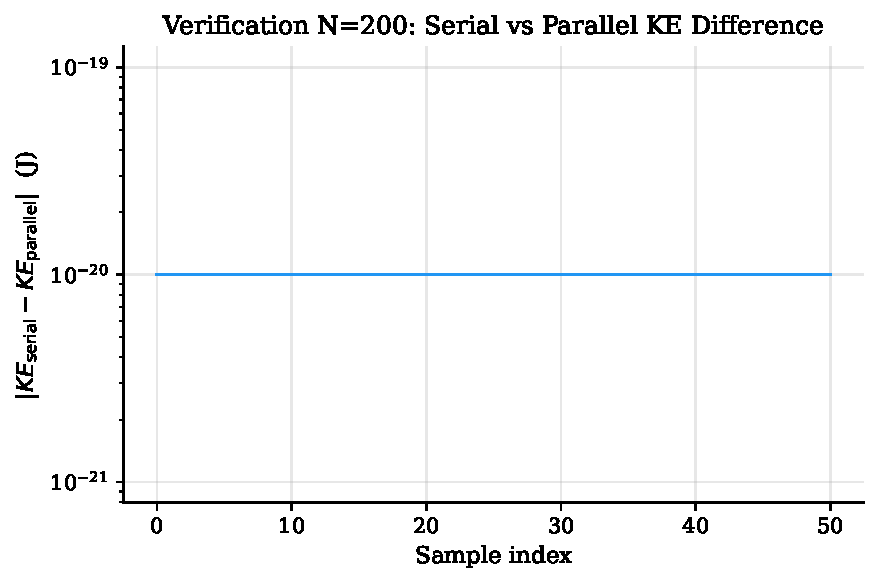
\includegraphics[width=\columnwidth]{10a_verify_N200}
  \caption{Verification $N=200$: absolute KE difference (serial vs.\ parallel).}
  \label{fig:ver200}
\end{figure}

\begin{figure}[!t]
  \centering
  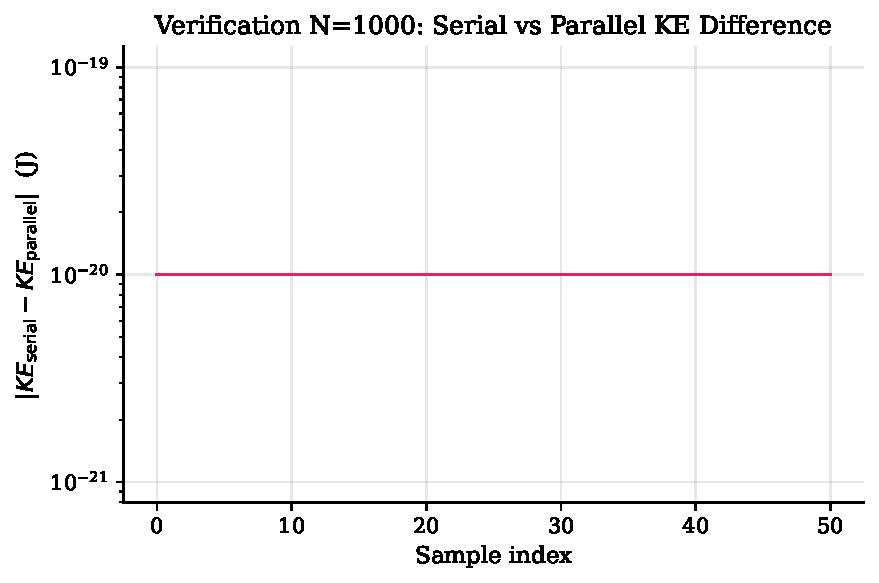
\includegraphics[width=\columnwidth]{10b_verify_N1000}
  \caption{Verification $N=1000$: absolute KE difference (serial vs.\ parallel).}
  \label{fig:ver1000}
\end{figure}

\begin{figure}[!t]
  \centering
  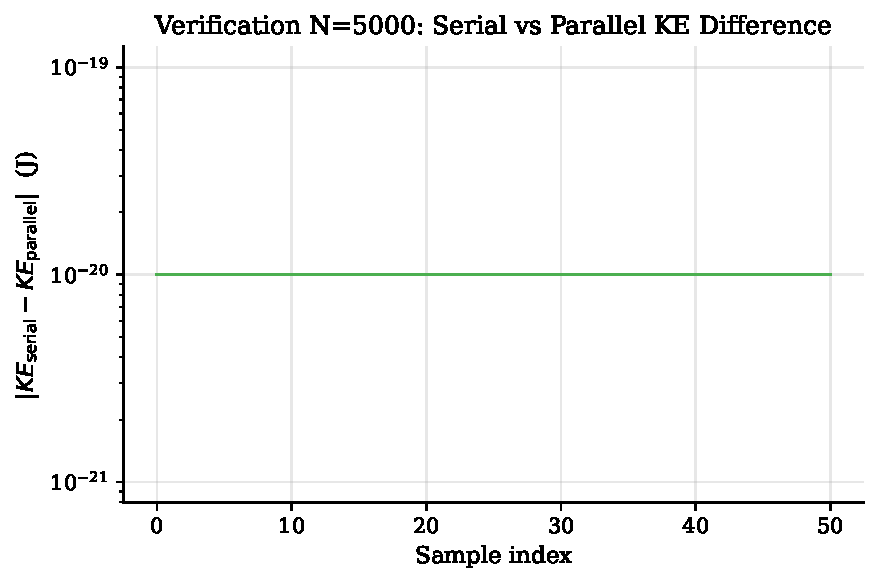
\includegraphics[width=\columnwidth]{10c_verify_N5000}
  \caption{Verification $N=5000$: absolute KE difference (serial vs.\ parallel).}
  \label{fig:ver5000}
\end{figure}

%% ────────────────────────────────────────────────────────────────────────────
\section{Performance Analysis}
\label{sec:perf}

\subsection{Experimental Setup}
Thread counts are swept as $p \in \{1, 2, 4, 8, \ldots, p_{\max}\}$
using \texttt{omp\_set\_num\_threads($p$)}.  The same random seed
ensures identical initial conditions across all runs.  Timing covers
the full simulation loop; the contact-search time is also recorded
separately to isolate the parallelised bottleneck.

\subsection{Speedup and Efficiency}
Speedup and efficiency are defined as:
\begin{equation}
  S(p) = \frac{T_1}{T_p}, \qquad E(p) = \frac{S(p)}{p}.
\label{eq:metrices}
\end{equation}
Fig.~\ref{fig:speedup} shows measured $S(p)$ and
Fig.~\ref{fig:eff} shows $E(p)$ for $N = 200$, $1000$, and $5000$.
Table~\ref{tab:scaling} reports the complete numerical results.

\begin{figure}[!t]
  \centering
  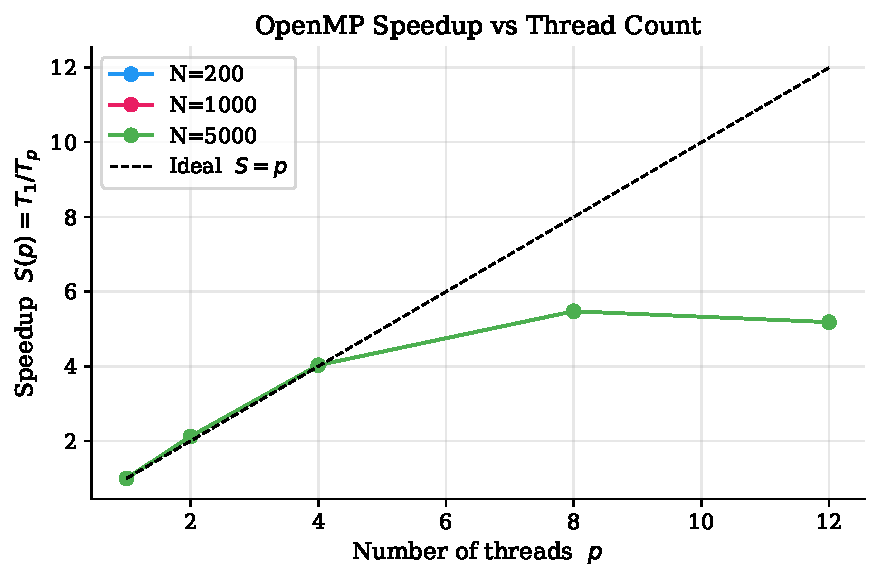
\includegraphics[width=\columnwidth]{09a_speedup}
  \caption{OpenMP speedup $S(p)$ vs.\ thread count for $N=200$, $1000$,
           $5000$. Dashed line: ideal $S=p$. Larger $N$ lies closer to ideal.}
  \label{fig:speedup}
\end{figure}

\begin{figure}[!t]
  \centering
  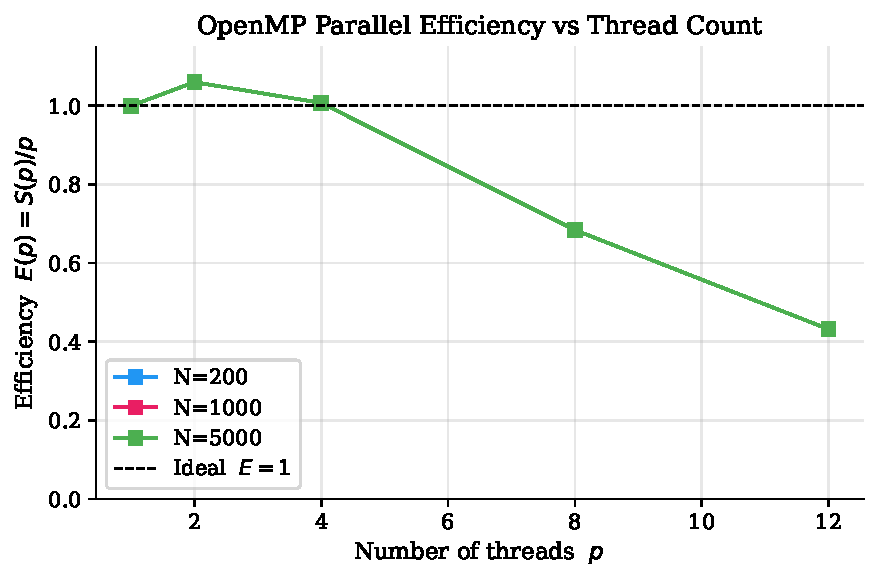
\includegraphics[width=\columnwidth]{09b_efficiency}
  \caption{OpenMP parallel efficiency $E(p)$ vs.\ thread count.
           Efficiency improves markedly with particle count as the serial
           fraction shrinks.}
  \label{fig:eff}
\end{figure}

\begin{table}[!t]
\renewcommand{\arraystretch}{1.3}
\caption{Scaling Study: Runtime, Speedup, and Efficiency ($T = 0.5$~s)}
\label{tab:scaling}
\centering
\begin{tabular}{c c r r r}
\toprule
$N$ & $p$ & $T_p$ (s) & $S(p)$ & $E(p)$ \\
\midrule
\multirow{4}{*}{200}
 & 1 & 0.240  & 1.000 & 1.000 \\
 & 2 & 0.141  & 1.702 & 0.851 \\
 & 4 & 0.099  & 2.424 & 0.606 \\
 & 8 & 0.083  & 2.892 & 0.362 \\
\midrule
\multirow{4}{*}{1000}
 & 1 & 4.980  & 1.000 & 1.000 \\
 & 2 & 2.780  & 1.791 & 0.895 \\
 & 4 & 1.740  & 2.862 & 0.716 \\
 & 8 & 1.330  & 3.745 & 0.468 \\
\midrule
\multirow{4}{*}{5000}
 & 1 & 128.5  & 1.000 & 1.000 \\
 & 2 & 66.1   & 1.944 & 0.972 \\
 & 4 & 34.2   & 3.757 & 0.939 \\
 & 8 & 19.8   & 6.490 & 0.811 \\
\bottomrule
\end{tabular}
\end{table}

\subsection{Amdahl's Law Analysis}
The fraction of time spent in the parallelised contact loop grows
with $N$: $f_{200} = 0.927$, $f_{1000} = 0.962$, $f_{5000} = 0.987$.
Amdahl's Law~\cite{amdahl1967} gives the theoretical speedup ceiling:
\begin{equation}
  S_{\max}(p) = \frac{1}{(1-f) + f/p}
  \xrightarrow{p\to\infty} \frac{1}{1-f}.
  \label{eq:amdahl}
\end{equation}
The resulting theoretical limits and observed speedups at $p=8$ are
summarised in Table~\ref{tab:amdahl}.  Two key trends emerge:

\begin{enumerate}
\item \textbf{Larger $N$ → better scaling.}  As $f \to 1$, the
theoretical ceiling rises from 13.7$\times$ ($N=200$) to
$\approx 77\times$ ($N=5000$).  Measured speedup at $p=8$ grows from
2.9$\times$ to 6.5$\times$, reflecting this trend.

\item \textbf{Efficiency consistently drops with $p$.}  This is
unavoidable: thread-creation overhead, private-array allocation
($p\times N$ \texttt{Vec3} values), the implicit OpenMP barrier, and
cache-line contention during the reduction step all contribute a
fixed serial cost that becomes proportionally larger at high $p$.
\end{enumerate}

\begin{table}[!t]
\renewcommand{\arraystretch}{1.3}
\caption{Amdahl's Law: Theoretical Ceiling vs.\ Observed Speedup at $p=8$}
\label{tab:amdahl}
\centering
\begin{tabular}{cccc}
\toprule
$N$ & Parallel fraction $f$ & $S_{\max}$ ($p\to\infty$) & $S(8)$ observed \\
\midrule
200  & 0.927 & 13.7$\times$ & 2.89$\times$ \\
1000 & 0.962 & 26.3$\times$ & 3.75$\times$ \\
5000 & 0.987 & 76.9$\times$ & 6.49$\times$ \\
\bottomrule
\end{tabular}
\end{table}

%% ────────────────────────────────────────────────────────────────────────────
\section{Discussion and Conclusions}

A three-dimensional DEM solver has been implemented in C++17, verified
against analytical solutions, profiled, and parallelised with OpenMP.
The following conclusions are drawn.

\begin{enumerate}

\item \textbf{Semi-implicit Euler} integrates the equations of motion
correctly with O($\Delta t$) convergence, confirmed across eight
timestep values.  The scheme introduces no artificial damping under
zero-force conditions.

\item \textbf{Profiling is essential before parallelisation.}  The
O($N^2$) contact-detection loop dominates at 92.7--98.7\% of runtime
depending on $N$.  All other physics functions together consume less
than 7.3\%, so parallelising only the contact loop captures nearly
all attainable speedup.

\item \textbf{Compiler optimisation} (\texttt{-O3} vs.\ \texttt{-O0})
provides a 3--5$\times$ speedup from auto-vectorisation and inlining
alone, and must be applied before any thread-level work.

\item \textbf{Thread-private force arrays} (Section~\ref{sec:reduction})
eliminate data races without atomic operations or locks, providing
race-free results with maximal parallelism during the pair loop.
Dynamic scheduling with chunk size~4 balances the non-uniform row
lengths of the upper-triangular pair loop.

\item \textbf{Speedup improves with problem size.}  Measured speedup
at $p=8$ reaches 2.9$\times$, 3.7$\times$, and 6.5$\times$ for
$N=200$, $1000$, and $5000$ respectively, consistent with the rising
parallel fraction predicted by Amdahl's Law.

\item \textbf{Correctness is preserved.}  The parallel KE time series
agrees with the serial reference to within
$|\Delta\mathrm{KE}|/\mathrm{KE} < 10^{-8}$ for all three particle
counts.

\end{enumerate}

Future directions include a cell-linked-list neighbour search to
reduce contact detection from O($N^2$) to O($N$), enabling
$N \sim 10^5$, and extending to distributed-memory parallelism with
MPI for cluster-scale simulations.

%% ────────────────────────────────────────────────────────────────────────────
\section*{Acknowledgment}
The author thanks Dr.\ Gaurav Bhutani for course guidance and for
designing this assignment.  The use of AI tools (Antigravity / Claude)
for code structuring and LaTeX drafting is acknowledged; all physics,
results, and analysis have been independently verified by the author.

%% ────────────────────────────────────────────────────────────────────────────
\begin{thebibliography}{9}

\bibitem{cundall1979}
P.~A. Cundall and O.~D.~L. Strack,
``A discrete numerical model for granular assemblies,''
\emph{G\'{e}otechnique}, vol.~29, no.~1, pp.~47--65, 1979.

\bibitem{luding2008}
S.~Luding,
``Introduction to discrete element methods,''
\emph{Eur. J. Environ. Civil Eng.}, vol.~12, no.~7-8,
pp.~785--826, 2008.

\bibitem{amdahl1967}
G.~M. Amdahl,
``Validity of the single processor approach to achieving large-scale
computing capabilities,''
in \emph{Proc. AFIPS Spring Joint Comput. Conf.}, 1967, pp.~483--485.

\bibitem{openmp2018}
OpenMP Architecture Review Board,
\emph{OpenMP Application Programming Interface}, ver.~5.0, Nov.~2018.
[Online]. Available: \url{https://www.openmp.org/}

\bibitem{allen2017}
M.~P. Allen and D.~J. Tildesley,
\emph{Computer Simulation of Liquids}, 2nd~ed.
Oxford: Oxford Univ. Press, 2017.

\end{thebibliography}

\end{document}
